\begin{center}
	\section*{APPENDICES}
\end{center}
\addcontentsline{toc}{section}{\textbf{APPENDICES }}
\renewcommand{\thepage}{\arabic{page}}

\begin{landscape}
	\begin{table}[ht]
		\caption*{Appendix Table 1: VDC-wise variables used for the construction of Household Vulnerability Index}
		\renewcommand{\arraystretch}{1.2}
		\resizebox{1.8\textwidth}{!}{%
			\begin{tabular}{lcccccccccccc}
				\hline
				\multirow{3}{*}{\textbf{\begin{tabular}[c]{@{}l@{}}Year/\\ District/\\ VDC\end{tabular}}} & \multicolumn{4}{c}{\textbf{2006}}                                                                                                                                                                                                                               & \multicolumn{4}{c}{\textbf{2009}}                                                                                                                                                                                                                               & \multicolumn{4}{c}{\textbf{2012}}                                                                                                                                                                                                                               \\ \hline
				& \textbf{Chitwan}                                              & \textbf{Kaski}                                                & \multicolumn{2}{c}{\textbf{Mustang}}                                                                                            & \textbf{Chitwan}                                              & \textbf{Kaski}                                                & \multicolumn{2}{c}{\textbf{Mustang}}                                                                                            & \textbf{Chitwan}                                              & \textbf{Kaski}                                                & \multicolumn{2}{c}{\textbf{Mustang}}                                                                                            \\ \hline
				& \textbf{Chainpur}                                             & \textbf{Hemja}                                                & \textbf{Kunjo}                                                 & \textbf{Lete}                                                  & \textbf{Chainpur}                                             & \textbf{Hemja}                                                & \textbf{Kunjo}                                                 & \textbf{Lete}                                                  & \textbf{Chainpur}                                             & \textbf{Hemja}                                                & \textbf{Kunjo}                                                 & \textbf{Lete}                                                  \\ \hline
				\multicolumn{13}{l}{\textbf{Human Capital}}                                                                                                                                                                                                                                                                                                                                                                                                                                                                                                                                                                                                                                                                                                                                                                                                                                                     \\
				HHH Age                                                                                   & \begin{tabular}[c]{@{}c@{}}50.36\\  (14.15)\end{tabular}      & \begin{tabular}[c]{@{}c@{}}50.14 \\ (14.57)\end{tabular}      & \begin{tabular}[c]{@{}c@{}}51.54\\  (14.66)\end{tabular}       & \begin{tabular}[c]{@{}c@{}}54.16 \\ (12.32)\end{tabular}       & \begin{tabular}[c]{@{}c@{}}52.13 \\ (13.75)\end{tabular}      & \begin{tabular}[c]{@{}c@{}}52.00 \\ (13.39)\end{tabular}      & \begin{tabular}[c]{@{}c@{}}52.63\\ (14.57)\end{tabular}        & \begin{tabular}[c]{@{}c@{}}55.50\\ (12.95)\end{tabular}        & \begin{tabular}[c]{@{}c@{}}52.24\\ (17.20)\end{tabular}       & \begin{tabular}[c]{@{}c@{}}53.52\\ (13.71)\end{tabular}       & \begin{tabular}[c]{@{}c@{}}52.77\\ (15.92)\end{tabular}        & \begin{tabular}[c]{@{}c@{}}57.54\\ (11.98)\end{tabular}        \\
				HH head Education                                                                         & \begin{tabular}[c]{@{}c@{}}3.08\\ (4.06)\end{tabular}         & \begin{tabular}[c]{@{}c@{}}6.29\\ (4.97)\end{tabular}         & \begin{tabular}[c]{@{}c@{}}2.83\\ (3.42)\end{tabular}          & \begin{tabular}[c]{@{}c@{}}3.25\\ (4.46)\end{tabular}          & \begin{tabular}[c]{@{}c@{}}2.93\\ (4.06)\end{tabular}         & \begin{tabular}[c]{@{}c@{}}6.07\\ (5.23)\end{tabular}         & \begin{tabular}[c]{@{}c@{}}2.79\\ (3.28)\end{tabular}          & \begin{tabular}[c]{@{}c@{}}3.08\\ (4.21)\end{tabular}          & \begin{tabular}[c]{@{}c@{}}2.91\\ (4.33)\end{tabular}         & \begin{tabular}[c]{@{}c@{}}6.91\\ (5.07)\end{tabular}         & \begin{tabular}[c]{@{}c@{}}2.48\\ (3.39)\end{tabular}          & \begin{tabular}[c]{@{}c@{}}3.30\\ (4.62)\end{tabular}          \\
				Max HH Education                                                                          & \begin{tabular}[c]{@{}c@{}}8.44\\ (3.91)\end{tabular}         & \begin{tabular}[c]{@{}c@{}}10.76\\ (2.90)\end{tabular}        & \begin{tabular}[c]{@{}c@{}}7.10\\ (2.92)\end{tabular}          & \begin{tabular}[c]{@{}c@{}}8.14\\ (3.60)\end{tabular}          & \begin{tabular}[c]{@{}c@{}}9.70\\ (3.63)\end{tabular}         & \begin{tabular}[c]{@{}c@{}}11.18\\ (3.94)\end{tabular}        & \begin{tabular}[c]{@{}c@{}}7.75\\ (3.47)\end{tabular}          & \begin{tabular}[c]{@{}c@{}}8.32\\ (4.33)\end{tabular}          & \begin{tabular}[c]{@{}c@{}}9.89\\ (4.44)\end{tabular}         & \begin{tabular}[c]{@{}c@{}}11.91\\ (4.03)\end{tabular}        & \begin{tabular}[c]{@{}c@{}}7.72\\ (3.71)\end{tabular}          & \begin{tabular}[c]{@{}c@{}}8.70\\ (3.97)\end{tabular}          \\
				\multicolumn{13}{l}{\textbf{Physical Capital}}                                                                                                                                                                                                                                                                                                                                                                                                                                                                                                                                                                                                                                                                                                                                                                                                                                                  \\
				Total Implements                                                                          & \begin{tabular}[c]{@{}c@{}}4660.32\\ (11275.49)\end{tabular}  & \begin{tabular}[c]{@{}c@{}}14057.03\\ (16860.42)\end{tabular} & \begin{tabular}[c]{@{}c@{}}6579.07\\ (11240.12)\end{tabular}   & \begin{tabular}[c]{@{}c@{}}13892.80\\ (24616.53)\end{tabular}  & \begin{tabular}[c]{@{}c@{}}10153.80\\ (23970.94)\end{tabular} & \begin{tabular}[c]{@{}c@{}}30700.02\\ (46128.36)\end{tabular} & \begin{tabular}[c]{@{}c@{}}11694.79\\ (16393.21)\end{tabular}  & \begin{tabular}[c]{@{}c@{}}18349.19\\ (31531.21)\end{tabular}  & \begin{tabular}[c]{@{}c@{}}22165.29\\ (38089.25)\end{tabular} & \begin{tabular}[c]{@{}c@{}}48959.02\\ (70582.56)\end{tabular} & \begin{tabular}[c]{@{}c@{}}19824.44\\ (30068.34)\end{tabular}  & \begin{tabular}[c]{@{}c@{}}23000.68\\ (25109.33)\end{tabular}  \\
				Total Livestock                                                                           & \begin{tabular}[c]{@{}c@{}}18532.68\\ (15428.31)\end{tabular} & \begin{tabular}[c]{@{}c@{}}26573.08\\ (20411.58)\end{tabular} & \begin{tabular}[c]{@{}c@{}}64484.18\\ (217769.73)\end{tabular} & \begin{tabular}[c]{@{}c@{}}95156.95\\ (230659.93)\end{tabular} & \begin{tabular}[c]{@{}c@{}}43936.83\\ (39679.84)\end{tabular} & \begin{tabular}[c]{@{}c@{}}35690.11\\ (35760.07)\end{tabular} & \begin{tabular}[c]{@{}c@{}}48328.19\\ (157785.27)\end{tabular} & \begin{tabular}[c]{@{}c@{}}63305.51\\ (196365.44)\end{tabular} & \begin{tabular}[c]{@{}c@{}}38993.71\\ (34330.40)\end{tabular} & \begin{tabular}[c]{@{}c@{}}34635.84\\ (39306.60)\end{tabular} & \begin{tabular}[c]{@{}c@{}}43044.51\\ (40803.87)\end{tabular}  & \begin{tabular}[c]{@{}c@{}}25772.02\\ (36222.90)\end{tabular}  \\
				Total Land owned\\
				(in sq. m)                                                               & \begin{tabular}[c]{@{}c@{}}2027.47\\ (6367.27)\end{tabular}   & \begin{tabular}[c]{@{}c@{}}1187.00\\ (1013.02)\end{tabular}   & \begin{tabular}[c]{@{}c@{}}2851.25\\ (2588.66)\end{tabular}    & \begin{tabular}[c]{@{}c@{}}3023.66\\ (2979.45)\end{tabular}    & \begin{tabular}[c]{@{}c@{}}915.91\\ (765.38)\end{tabular}     & \begin{tabular}[c]{@{}c@{}}1491.41\\ (2060.25)\end{tabular}   & \begin{tabular}[c]{@{}c@{}}2443.77\\ (4381.85)\end{tabular}    & \begin{tabular}[c]{@{}c@{}}2040.13\\ (3034.05)\end{tabular}    & \begin{tabular}[c]{@{}c@{}}1041.46\\ (1136.88)\end{tabular}   & \begin{tabular}[c]{@{}c@{}}1374.96\\ (2253.95)\end{tabular}   & \begin{tabular}[c]{@{}c@{}}2120.03\\ (1955.97)\end{tabular}    & \begin{tabular}[c]{@{}c@{}}1734.96\\ (1825.09)\end{tabular}    \\
				\multicolumn{13}{l}{\textbf{Social Capital}}                                                                                                                                                                                                                                                                                                                                                                                                                                                                                                                                                                                                                                                                                                                                                                                                                                                    \\
				HH belong to \\ biggest caste                                                                & \begin{tabular}[c]{@{}c@{}}0.58\\ (0.50)\end{tabular}         & \begin{tabular}[c]{@{}c@{}}0.89\\ (0.32)\end{tabular}         & \begin{tabular}[c]{@{}c@{}}0.44\\ (0.50)\end{tabular}          & \begin{tabular}[c]{@{}c@{}}0.54\\ (0.50)\end{tabular}          & \begin{tabular}[c]{@{}c@{}}0.66\\ (0.48)\end{tabular}         & \begin{tabular}[c]{@{}c@{}}0.98\\ (0.14)\end{tabular}         & \begin{tabular}[c]{@{}c@{}}0.52\\ (0.50)\end{tabular}          & \begin{tabular}[c]{@{}c@{}}0.63\\ (0.49)\end{tabular}          & \begin{tabular}[c]{@{}c@{}}0.50\\ (0.50)\end{tabular}         & \begin{tabular}[c]{@{}c@{}}0.86\\ (0.50)\end{tabular}         & \begin{tabular}[c]{@{}c@{}}0.50\\ (0.35)\end{tabular}          & \begin{tabular}[c]{@{}c@{}}0.68\\ (0.47)\end{tabular}          \\
				\multicolumn{13}{l}{\textbf{Financial Capital}}                                                                                                                                                                                                                                                                                                                                                                                                                                                                                                                                                                                                                                                                                                                                                                                                                                                 \\
				Bank Saving                                                                               & \begin{tabular}[c]{@{}c@{}}879.58\\ (2661.50)\end{tabular}    & \begin{tabular}[c]{@{}c@{}}9663.83\\ (26812.62)\end{tabular}  & \begin{tabular}[c]{@{}c@{}}26550.42\\ (49925.24)\end{tabular}  & \begin{tabular}[c]{@{}c@{}}36893.08\\ (100295.99)\end{tabular} & \begin{tabular}[c]{@{}c@{}}1911.63\\ (6126.69)\end{tabular}   & \begin{tabular}[c]{@{}c@{}}11937.72\\ (31025.90)\end{tabular} & \begin{tabular}[c]{@{}c@{}}15583.53\\ (33746.90)\end{tabular}  & \begin{tabular}[c]{@{}c@{}}32899.60\\ (75131.34)\end{tabular}  & \begin{tabular}[c]{@{}c@{}}11953.55\\ (31763.88)\end{tabular} & \begin{tabular}[c]{@{}c@{}}25410.64\\ (66932.34)\end{tabular} & \begin{tabular}[c]{@{}c@{}}24116.56\\ (64770.84)\end{tabular}  & \begin{tabular}[c]{@{}c@{}}70411.25\\ (127638.23)\end{tabular} \\
				Jewellery                                                                                 & \begin{tabular}[c]{@{}c@{}}0.00\\ (0.00)\end{tabular}         & \begin{tabular}[c]{@{}c@{}}0.00\\ (0.00)\end{tabular}         & \begin{tabular}[c]{@{}c@{}}17329.52\\ (31072.47)\end{tabular}  & \begin{tabular}[c]{@{}c@{}}45053.31\\ (87655.54)\end{tabular}  & \begin{tabular}[c]{@{}c@{}}4396.88\\ (6965.53)\end{tabular}   & \begin{tabular}[c]{@{}c@{}}20485.87\\ (16594.26)\end{tabular} & \begin{tabular}[c]{@{}c@{}}25209.19\\ (56538.65)\end{tabular}  & \begin{tabular}[c]{@{}c@{}}51106.62\\ (94727.93)\end{tabular}  & \begin{tabular}[c]{@{}c@{}}21477.20\\ (23620.47)\end{tabular} & \begin{tabular}[c]{@{}c@{}}51605.94\\ (48463.62)\end{tabular} & \begin{tabular}[c]{@{}c@{}}45374.61\\ (120899.24)\end{tabular} & \begin{tabular}[c]{@{}c@{}}62313.92\\ (103824.98)\end{tabular} \\
				\textbf{Livelihood}                                                                       & \multicolumn{1}{l}{}                                          & \multicolumn{1}{l}{}                                          & \multicolumn{1}{l}{}                                           & \multicolumn{1}{l}{}                                           & \multicolumn{1}{l}{}                                          & \multicolumn{1}{l}{}                                          & \multicolumn{1}{l}{}                                           & \multicolumn{1}{l}{}                                           & \multicolumn{1}{l}{}                                          & \multicolumn{1}{l}{}                                          & \multicolumn{1}{l}{}                                           & \multicolumn{1}{l}{}                                           \\
				No. of livelihood strategies                                                              & \begin{tabular}[c]{@{}c@{}}4.81\\ (0.97)\end{tabular}         & \begin{tabular}[c]{@{}c@{}}4.72\\ (0.91)\end{tabular}         & \begin{tabular}[c]{@{}c@{}}4.80\\ (0.92)\end{tabular}          & \begin{tabular}[c]{@{}c@{}}4.32\\ (0.93)\end{tabular}          & \begin{tabular}[c]{@{}c@{}}4.93\\ (1.02)\end{tabular}         & \begin{tabular}[c]{@{}c@{}}4.74\\ (0.91)\end{tabular}         & \begin{tabular}[c]{@{}c@{}}5.35\\ (0.83)\end{tabular}          & \begin{tabular}[c]{@{}c@{}}4.86\\ (0.86)\end{tabular}          & \begin{tabular}[c]{@{}c@{}}4.60\\ (0.98)\end{tabular}         & \begin{tabular}[c]{@{}c@{}}4.78\\ (0.90)\end{tabular}         & \begin{tabular}[c]{@{}c@{}}4.76\\ (0.87)\end{tabular}          & \begin{tabular}[c]{@{}c@{}}4.45\\ (1.10)\end{tabular}          \\
				\textbf{Household Vulnerability}                                                          &                                                               &                                                               &                                                                &                                                                &                                                               &                                                               &                                                                &                                                                &                                                               &                                                               &                                                                &                                                                \\
				HVI                                                                                       & \begin{tabular}[c]{@{}c@{}}0.62\\ (0.05)\end{tabular}         & \begin{tabular}[c]{@{}c@{}}0.62\\ (0.04)\end{tabular}         & \begin{tabular}[c]{@{}c@{}}0.65\\ (0.05)\end{tabular}          & \begin{tabular}[c]{@{}c@{}}0.63\\ (0.05)\end{tabular}          & \begin{tabular}[c]{@{}c@{}}0.61\\ (0.05)\end{tabular}         & \begin{tabular}[c]{@{}c@{}}0.62\\ (0.04)\end{tabular}         & \begin{tabular}[c]{@{}c@{}}0.64\\ (0.05)\end{tabular}          & \begin{tabular}[c]{@{}c@{}}0.63\\ (0.05)\end{tabular}          & \begin{tabular}[c]{@{}c@{}}0.61\\ (0.05)\end{tabular}         & \begin{tabular}[c]{@{}c@{}}0.62\\ (0.05)\end{tabular}         & \begin{tabular}[c]{@{}c@{}}0.64\\ (0.05)\end{tabular}          & \begin{tabular}[c]{@{}c@{}}0.62\\ (0.05)\end{tabular}       \\  \hline \hline
			\end{tabular}
		}
		\textit{Note: Standard deviation in the parenthesis \\
			Source: Author's calculation}
	\end{table}
\end{landscape}

\begin{landscape}
	\begin{center}
		\begin{table}[ht]
			\captionsetup{labelformat=empty}
			\caption*{Appendix Table 2: Mean and SD of the Components used in HVI Construction}
			\label{tab:MeanandSDofComponentsusedinHVIConstruction}
			\resizebox{1.7\textwidth}{!}{%
				\begin{tabular}{lcccccccccccc} \hline
					& \multicolumn{4}{c}{\textbf{2006}}                                                                                                                                                                                                                    & \multicolumn{4}{c}{\textbf{2009}}                                                                                                                                                                                             & \multicolumn{4}{c}{\textbf{2012}}                                                                                                                                                                                             \\ \hline
					& \textbf{Chitwan}                                                             & \textbf{Kaski}                                        & \multicolumn{2}{c}{\textbf{Mustang}}                                                                          & \textbf{Chitwan}                                      & \textbf{Kaski}                                        & \multicolumn{2}{c}{\textbf{Mustang}}                                                                          & \textbf{Chitwan}                                      & \textbf{Kaski}                                        & \multicolumn{2}{c}{\textbf{Mustang}}                                                                          \\ \hline
					\multirow{-3}{*}{\textbf{\begin{tabular}[c]{@{}c@{}}Year/\\ District/\\ VDC\end{tabular}}} & \textbf{Chainpur}                                                            & \textbf{Hemja}                                        & \textbf{Kunjo}                                        & \textbf{Lete}                                         & \textbf{Chainpur}                                     & \textbf{Hemja}                                        & \textbf{Kunjo}                                        & \textbf{Lete}                                         & \textbf{Chainpur}                                     & \textbf{Hemja}                                        & \textbf{Kunjo}                                        & \textbf{Lete}                                         \\ \hline
					\textbf{\begin{tabular}[c]{@{}c@{}}Human Capital (C1)\end{tabular}}                     & \begin{tabular}[c]{@{}c@{}}0.48\\ (0.11)\end{tabular}                        & \begin{tabular}[c]{@{}c@{}}0.49\\ (0.11)\end{tabular} & \begin{tabular}[c]{@{}c@{}}0.48\\ (0.09)\end{tabular} & \begin{tabular}[c]{@{}c@{}}0.47\\ (0.09)\end{tabular} & \begin{tabular}[c]{@{}c@{}}0.48\\ (0.11)\end{tabular} & \begin{tabular}[c]{@{}c@{}}0.48\\ (0.12)\end{tabular} & \begin{tabular}[c]{@{}c@{}}0.48\\ (0.09)\end{tabular} & \begin{tabular}[c]{@{}c@{}}0.48\\ (0.11)\end{tabular} & \begin{tabular}[c]{@{}c@{}}0.48\\ (0.10)\end{tabular} & \begin{tabular}[c]{@{}c@{}}0.48\\ (0.12)\end{tabular} & \begin{tabular}[c]{@{}c@{}}0.48\\ (0.10)\end{tabular} & \begin{tabular}[c]{@{}c@{}}0.45\\ (0.11)\end{tabular} \\
					\textbf{\begin{tabular}[c]{@{}c@{}}Physical Capital (C2)\end{tabular}}                   & \begin{tabular}[c]{@{}c@{}}0.98\\ (0.03)\end{tabular}                        & \begin{tabular}[c]{@{}c@{}}0.98\\ (0.01)\end{tabular} & \begin{tabular}[c]{@{}c@{}}0.97\\ (0.05)\end{tabular} & \begin{tabular}[c]{@{}c@{}}0.96\\ (0.05)\end{tabular} & \begin{tabular}[c]{@{}c@{}}0.98\\ (0.02)\end{tabular} & \begin{tabular}[c]{@{}c@{}}0.97\\ (0.04)\end{tabular} & \begin{tabular}[c]{@{}c@{}}0.97\\ (0.05)\end{tabular} & \begin{tabular}[c]{@{}c@{}}0.97\\ (0.05)\end{tabular} & \begin{tabular}[c]{@{}c@{}}0.97\\ (0.03)\end{tabular} & \begin{tabular}[c]{@{}c@{}}0.95\\ (0.05)\end{tabular} & \begin{tabular}[c]{@{}c@{}}0.97\\ (0.03)\end{tabular} & \begin{tabular}[c]{@{}c@{}}0.95\\ (0.02)\end{tabular} \\
					\textbf{\begin{tabular}[c]{@{}c@{}}Social Capital  (C3)\end{tabular}}                    & \begin{tabular}[c]{@{}c@{}}0.68\\ (0.33)\end{tabular}                        & \begin{tabular}[c]{@{}c@{}}0.84\\ (0.26)\end{tabular} & \begin{tabular}[c]{@{}c@{}}0.59\\ (0.35)\end{tabular} & \begin{tabular}[c]{@{}c@{}}0.66\\ (0.32)\end{tabular} & \begin{tabular}[c]{@{}c@{}}0.72\\ (0.32)\end{tabular} & \begin{tabular}[c]{@{}c@{}}0.87\\ (0.23)\end{tabular} & \begin{tabular}[c]{@{}c@{}}0.63\\ (0.32)\end{tabular} & \begin{tabular}[c]{@{}c@{}}0.69\\ (0.33)\end{tabular} & \begin{tabular}[c]{@{}c@{}}0.63\\ (0.33)\end{tabular} & \begin{tabular}[c]{@{}c@{}}0.62\\ (0.35)\end{tabular} & \begin{tabular}[c]{@{}c@{}}0.82\\ (0.27)\end{tabular} & \begin{tabular}[c]{@{}c@{}}0.70\\ (0.32)\end{tabular} \\
					\textbf{\begin{tabular}[c]{@{}c@{}}Livelihood  (C4)\end{tabular}}                        & \begin{tabular}[c]{@{}c@{}}0.99\\ (0.00)\end{tabular}                        & \begin{tabular}[c]{@{}c@{}}0.99\\ (0.01)\end{tabular} & \begin{tabular}[c]{@{}c@{}}0.97\\ (0.03)\end{tabular} & \begin{tabular}[c]{@{}c@{}}0.96\\ (0.06)\end{tabular} & \begin{tabular}[c]{@{}c@{}}0.99\\ (0.00)\end{tabular} & \begin{tabular}[c]{@{}c@{}}0.98\\ (0.01)\end{tabular} & \begin{tabular}[c]{@{}c@{}}0.97\\ (0.03)\end{tabular} & \begin{tabular}[c]{@{}c@{}}0.96\\ (0.05)\end{tabular} & \begin{tabular}[c]{@{}c@{}}0.98\\ (0.03)\end{tabular} & \begin{tabular}[c]{@{}c@{}}0.96\\ (0.03)\end{tabular} & \begin{tabular}[c]{@{}c@{}}0.96\\ (0.06)\end{tabular} & \begin{tabular}[c]{@{}c@{}}0.94\\ (0.06)\end{tabular} \\
					\textbf{\begin{tabular}[c]{@{}c@{}}Financial Capital  (C4)\end{tabular}}              & \begin{tabular}[c]{@{}c@{}}0.31\\ (0.14)\end{tabular}                        & \begin{tabular}[c]{@{}c@{}}0.33\\ (0.13)\end{tabular} & \begin{tabular}[c]{@{}c@{}}0.31\\ (0.13)\end{tabular} & \begin{tabular}[c]{@{}c@{}}0.38\\ (0.13)\end{tabular} & \begin{tabular}[c]{@{}c@{}}0.30\\ (0.15)\end{tabular} & \begin{tabular}[c]{@{}c@{}}0.32\\ (0.13)\end{tabular} & \begin{tabular}[c]{@{}c@{}}0.24\\ (0.12)\end{tabular} & \begin{tabular}[c]{@{}c@{}}0.31\\ (0.12)\end{tabular} & \begin{tabular}[c]{@{}c@{}}0.34\\ (0.14)\end{tabular} & \begin{tabular}[c]{@{}c@{}}0.32\\ (0.13)\end{tabular} & \begin{tabular}[c]{@{}c@{}}0.32\\ (0.13)\end{tabular} & \begin{tabular}[c]{@{}c@{}}0.32\\ (0.15) \end{tabular} \\ \hline \hline 
				\end{tabular} \\
			} \\
			Note : The values are scaled using the mini-max and maxi-min method.
		\end{table}
	\end{center}
\end{landscape}

\begin{landscape}
	\begin{figure}[h] 
		\vspace{-100pt}
		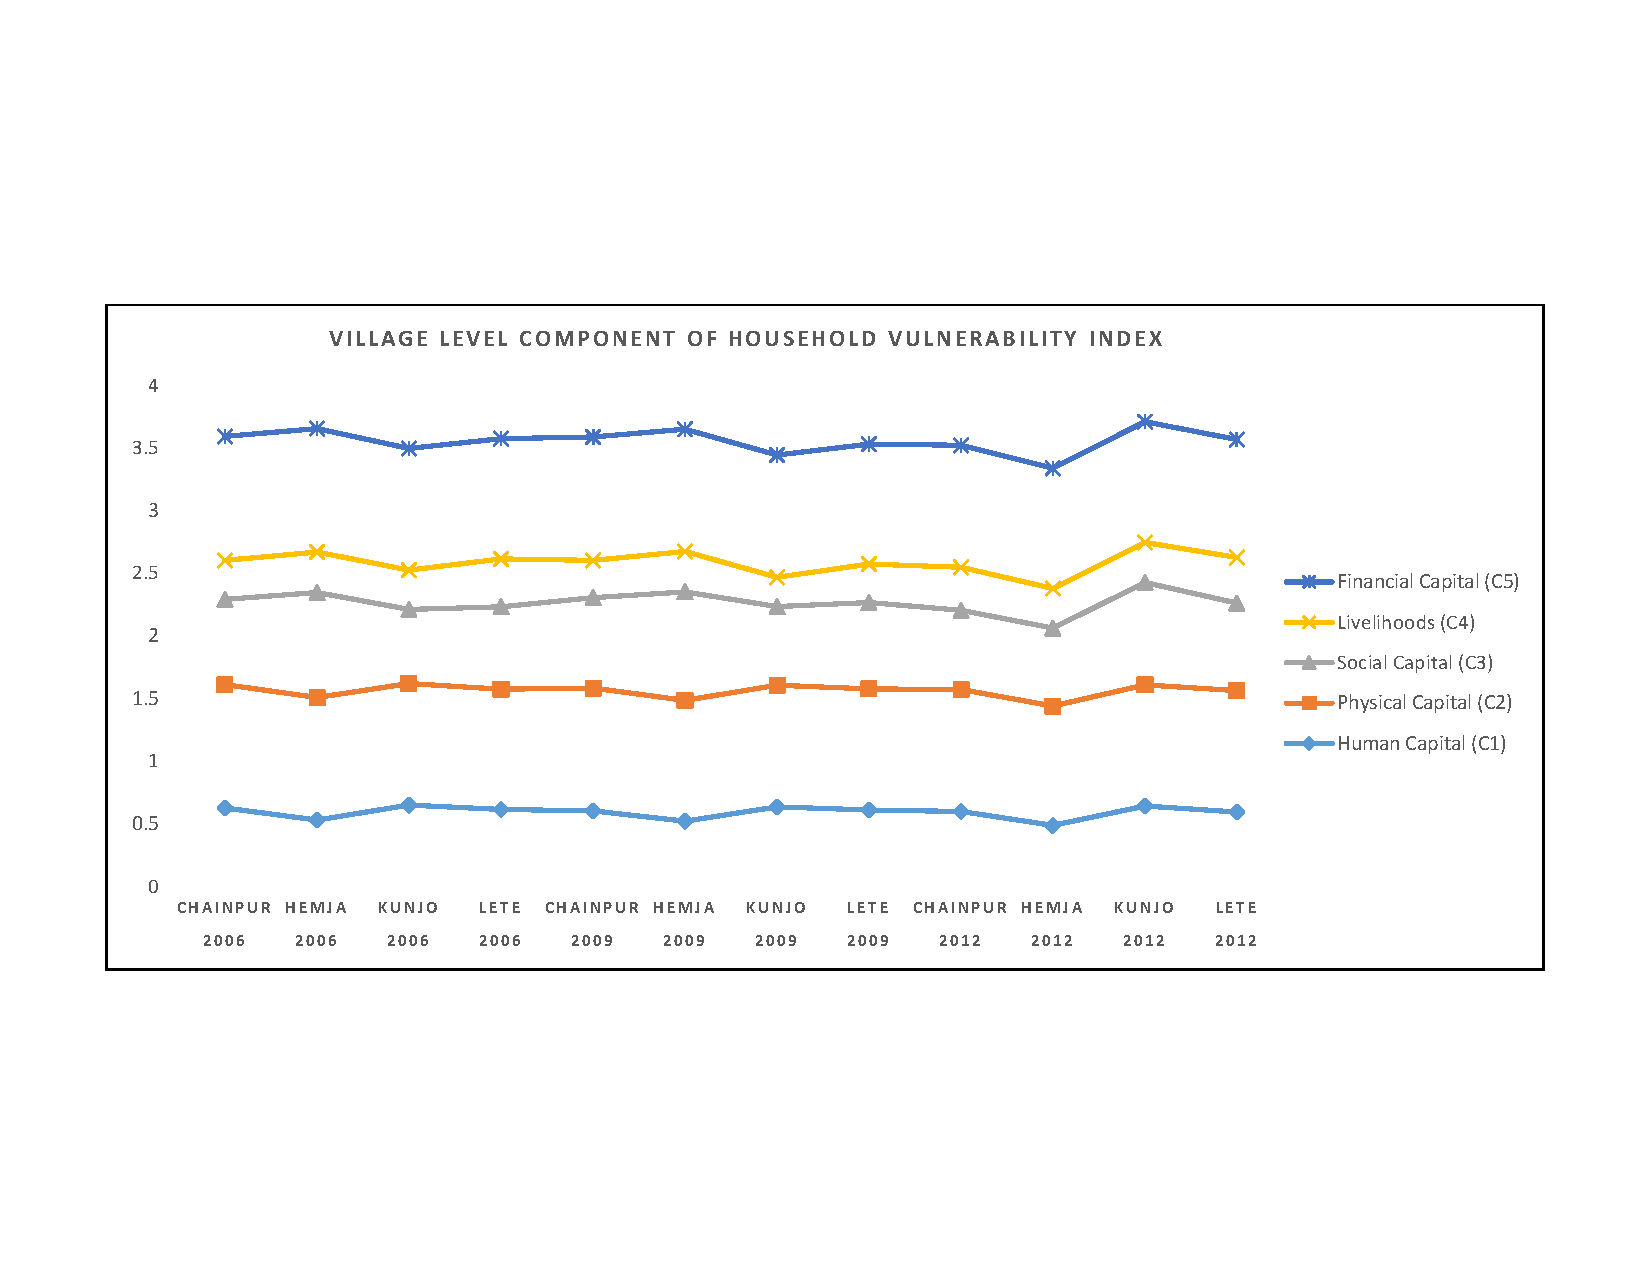
\includegraphics[scale=0.8]{Graphs and figures/HVI_Component_Village_Panel.pdf}
		\vspace{-50pt}
		\caption*{Appendix Fig 1: Village level HVI Components} 
		\label{fig:VDClevelhvicomponents}
		\captionsetup{skip=20pt}
	\end{figure}
\end{landscape}

\begin{table}[ht] 
	\captionsetup{labelformat=empty}
	\caption*{Appendix Table 3 : Pooled OLS Regression} 
	\label{} 
	\renewcommand{\arraystretch}{1.1}
	\resizebox{1.05\textwidth}{!}{%
		\begin{tabular}{@{\extracolsep{0.01pt}}lD{.}{.}{-3} D{.}{.}{-3} D{.}{.}{-3} D{.}{.}{-3} D{.}{.}{-3} D{.}{.}{-3} D{.}{.}{-3} } 
			\\[-1.6ex]\hline 
			\hline \\[-1.8ex] 
			& \multicolumn{7}{c}{\textit{Dependent variable:Household Vulnerability}} \\ 
			\cline{2-8} 		\\[-2.9ex] & \multicolumn{1}{c}{(1)} & \multicolumn{1}{c}{(2)} & \multicolumn{1}{c}{(3)} & \multicolumn{1}{c}{(4)} & \multicolumn{1}{c}{(5)} & \multicolumn{1}{c}{(6)} & \multicolumn{1}{c}{(7)}\\ 
			\hline \\[-1.8ex] 
			Env Dependence & 0.068^{***} & 0.068^{***} & 0.064^{***} & 0.062^{***} & 0.062^{***} & 0.049^{***} & 0.045^{***} \\ 
			& (0.012) & (0.012) & (0.012) & (0.012) & (0.012) & (0.012) & (0.012) \\ 
			& & & & & & & \\ 
			Debt &  & -0.001^{*} & -0.0004 & -0.0004 & -0.0004 & -0.0004 & -0.0005 \\ 
			&  & (0.0003) & (0.0003) & (0.0003) & (0.0003) & (0.0003) & (0.0003) \\ 
			& & & & & & & \\ 
			Depndency ratio &  &  & 0.022^{***} & 0.021^{***} & 0.021^{***} & 0.021^{***} & 0.020^{***} \\ 
			&  &  & (0.002) & (0.002) & (0.002) & (0.002) & (0.002) \\ 
			& & & & & & & \\ 
			Shock &  &  &  & 0.002^{*} & 0.002 & 0.001 & 0.001 \\ 
			&  &  &  & (0.001) & (0.001) & (0.001) & (0.001) \\ 
			& & & & & & & \\ 
			Constant & 0.557^{***} & 0.561^{***} & 0.550^{***} & 0.550^{***} & 0.552^{***} & 0.558^{***} & 0.562^{***} \\ 
			& (0.012) & (0.012) & (0.011) & (0.011) & (0.012) & (0.012) & (0.012) \\ 
			& & & & & & & \\ [-3.1ex]
			\hline \\[-2.5ex] 
			\textit{Fixed effects} & & & & & & & \\ 
			Year & \multicolumn{1}{c}{No} & \multicolumn{1}{c}{No} & \multicolumn{1}{c}{No} & \multicolumn{1}{c}{No} & \multicolumn{1}{c}{Yes} & \multicolumn{1}{c}{Yes} & \multicolumn{1}{c}{Yes} \\ 
			District & \multicolumn{1}{c}{No} & \multicolumn{1}{c}{No} & \multicolumn{1}{c}{No} & \multicolumn{1}{c}{No} & \multicolumn{1}{c}{No} & \multicolumn{1}{c}{Yes} & \multicolumn{1}{c}{Yes} \\ 
			VDC & \multicolumn{1}{c}{No} & \multicolumn{1}{c}{No} & \multicolumn{1}{c}{No} & \multicolumn{1}{c}{No} & \multicolumn{1}{c}{No} & \multicolumn{1}{c}{No} & \multicolumn{1}{c}{Yes} \\ 
			\hline \\[-2.5ex] 
			\textit{Fit statistics} & & & & & & & \\
			Observations & \multicolumn{1}{c}{1,284} & \multicolumn{1}{c}{1,284} & \multicolumn{1}{c}{1,284} & \multicolumn{1}{c}{1,284} & \multicolumn{1}{c}{1,284} & \multicolumn{1}{c}{1,284} & \multicolumn{1}{c}{1,284} \\ 
			R$^{2}$ & \multicolumn{1}{c}{0.024} & \multicolumn{1}{c}{0.027} & \multicolumn{1}{c}{0.105} & \multicolumn{1}{c}{0.107} & \multicolumn{1}{c}{0.108} & \multicolumn{1}{c}{0.126} & \multicolumn{1}{c}{0.131} \\ 
			Adjusted R$^{2}$ & \multicolumn{1}{c}{0.023} & \multicolumn{1}{c}{0.025} & \multicolumn{1}{c}{0.103} & \multicolumn{1}{c}{0.105} & \multicolumn{1}{c}{0.104} & \multicolumn{1}{c}{0.121} & \multicolumn{1}{c}{0.125} \\ 
			\hline 
			\hline \\[-1.8ex]  
		\end{tabular}
	}
	\textit{Note: Standard errors in the parenthesis} \hspace{2.52cm}{$^{*}$p$<$0.1; $^{**}$p$<$0.05; $^{***}$p$<$0.01} \\
	\textit{Env. = Environmental}
\end{table} 
\begin{table}[H] 
	\caption*{Appendix Table 4: Random Effects Regression} 
	\label{}
	\renewcommand{\arraystretch}{1.1}
	\resizebox{1.05\textwidth}{!}{% 
		\begin{tabular}{@{\extracolsep{0.01pt}}lD{.}{.}{-3} D{.}{.}{-3} D{.}{.}{-3} D{.}{.}{-3} D{.}{.}{-3} D{.}{.}{-3} D{.}{.}{-3} } 
			\\[-1.8ex]\hline 
			\hline \\[-2.9ex] 
			& \multicolumn{7}{c}{\textit{Dependent variable:Household Vulnerability}} \\ 
			\cline{2-8} \\[-7ex] 
			& \\
			[-1.8ex] & \multicolumn{1}{c}{(1)} & \multicolumn{1}{c}{(2)} & \multicolumn{1}{c}{(3)} & \multicolumn{1}{c}{(4)} & \multicolumn{1}{c}{(5)} & \multicolumn{1}{c}{(6)} & \multicolumn{1}{c}{(7)}\\ 
			\hline \\[-3.9ex] 
			Env. Dependence & 0.035^{***} & 0.035^{***} & 0.037^{***} & 0.035^{***} & 0.034^{***} & 0.026^{**} & 0.024^{**} \\ [-1.5ex]
			& (0.011) & (0.011) & (0.011) & (0.011) & (0.011) & (0.011) & (0.011) \\ [-3.5ex]
			& & & & & & & \\ 
			Debt &  & -0.001^{*} & -0.0003 & -0.0004 & -0.0004 & -0.0004 & -0.0004 \\ [-1.5ex]
			&  & (0.0003) & (0.0003) & (0.0003) & (0.0003) & (0.0003) & (0.0003) \\ [-3.5ex]
			& & & & & & & \\ 
			Dependency ratio &  &  & 0.020^{***} & 0.019^{***} & 0.019^{***} & 0.019^{***} & 0.018^{***} \\[-1.5ex] 
			&  &  & (0.002) & (0.002) & (0.002) & (0.002) & (0.002) \\ [-3.5ex]
			& & & & & & & \\ 
			Shock &  &  &  & 0.002^{**} & 0.001 & 0.001 & 0.001 \\ [-1.5ex]
			&  &  &  & (0.001) & (0.001) & (0.001) & (0.001) \\ [-3.5ex]
			& & & & & & & \\ 
			Constant & 0.588^{***} & 0.592^{***} & 0.576^{***} & 0.576^{***} & 0.580^{***} & 0.581^{***} & 0.583^{***} \\ [-1.5ex] 
			& (0.011) & (0.011) & (0.011) & (0.011) & (0.011) & (0.011) & (0.011) \\ [-4.5ex]
			& & & & & & & \\ 
			\hline \\[-5ex] 
			\textit{Fixed effects} & & & & & & & \\  \\[-6ex]
			Year & \multicolumn{1}{c}{No} & \multicolumn{1}{c}{No} & \multicolumn{1}{c}{No} & \multicolumn{1}{c}{No} & \multicolumn{1}{c}{Yes} & \multicolumn{1}{c}{Yes} & \multicolumn{1}{c}{Yes} \\ [-1.5ex]
			District & \multicolumn{1}{c}{No} & \multicolumn{1}{c}{No} & \multicolumn{1}{c}{No} & \multicolumn{1}{c}{No} & \multicolumn{1}{c}{No} & \multicolumn{1}{c}{Yes} & \multicolumn{1}{c}{Yes} \\ [-1.5ex]
			VDC & \multicolumn{1}{c}{No} & \multicolumn{1}{c}{No} & \multicolumn{1}{c}{No} & \multicolumn{1}{c}{No} & \multicolumn{1}{c}{No} & \multicolumn{1}{c}{No} & \multicolumn{1}{c}{Yes} \\ 
			\hline \\[-5ex] 
			\textit{Fit statistics} & & & & & & & \\ [-1.5ex]
			Observations & \multicolumn{1}{c}{1,284} & \multicolumn{1}{c}{1,284} & \multicolumn{1}{c}{1,284} & \multicolumn{1}{c}{1,284} & \multicolumn{1}{c}{1,284} & \multicolumn{1}{c}{1,284} & \multicolumn{1}{c}{1,284} \\ [-1.5ex]
			R$^{2}$ & \multicolumn{1}{c}{0.007} & \multicolumn{1}{c}{0.010} & \multicolumn{1}{c}{0.072} & \multicolumn{1}{c}{0.075} & \multicolumn{1}{c}{0.076} & \multicolumn{1}{c}{0.091} & \multicolumn{1}{c}{0.095} \\ [-1.5ex]
			Adjusted R$^{2}$ & \multicolumn{1}{c}{0.007} & \multicolumn{1}{c}{0.008} & \multicolumn{1}{c}{0.070} & \multicolumn{1}{c}{0.072} & \multicolumn{1}{c}{0.072} & \multicolumn{1}{c}{0.085} & \multicolumn{1}{c}{0.089} \\ 
			\hline 
			\hline \\[-2.6ex]  
		\end{tabular} 
	}
	\textit{Note: Standard errors in the parenthesis} \hspace{2.52cm}{$^{*}$p$<$0.1; $^{**}$p$<$0.05; $^{***}$p$<$0.01} \\ [-1.83ex]
	\textit{Env. = Environmental}
\end{table} 

\begin{table}[H] 
	\caption*{Appendix Table 5: Fixed Effects Regression} 
	\label{} 
	\renewcommand{\arraystretch}{1.1}
	\resizebox{1.05\textwidth}{!}{%
		\begin{tabular}{@{\extracolsep{5pt}}lD{.}{.}{-3} D{.}{.}{-3} D{.}{.}{-3} D{.}{.}{-3} D{.}{.}{-3} D{.}{.}{-3} D{.}{.}{-3} } 
			\\[-1.8ex]\hline 
			\hline \\[-3ex] 
			& \multicolumn{7}{c}{\textit{Dependent variable: Household Vulnerability}} \\ 
			\cline{2-8} 
			\\
			\\[-7.8ex] & \multicolumn{1}{c}{(1)} & \multicolumn{1}{c}{(2)} & \multicolumn{1}{c}{(3)} & \multicolumn{1}{c}{(4)} & \multicolumn{1}{c}{(5)} & \multicolumn{1}{c}{(6)} & \multicolumn{1}{c}{(7)}\\ 
			\hline \\[-3.98ex] 
			Env. Dependence & -0.003 & -0.003 & -0.001 & -0.001 & -0.004 & -0.004 & -0.004 \\ [-1.5ex]
			& (0.013) & (0.013) & (0.013) & (0.013) & (0.013) & (0.013) & (0.013) \\ [-3.5ex]
			& & & & & & & \\ 
			Debt &  & -0.0004 & -0.0003 & -0.0003 & -0.0003 & -0.0003 & -0.0003 \\ [-1.5ex]
			&  & (0.0004) & (0.0004) & (0.0004) & (0.0004) & (0.0004) & (0.0003) \\[-3.5ex] 
			& & & & & & & \\ 
			Dependency ratio &  &  & 0.015^{***} & 0.015^{***} & 0.014^{***} & 0.014^{***} & 0.014^{***} \\ [-1.5ex]
			&  &  & (0.003) & (0.003) & (0.003) & (0.003) & (0.002) \\ [-3.5ex]
			& & & & & & & \\ 
			Shock &  &  &  & 0.002^{*} & 0.001 & 0.001 & 0.001 \\ [-1.5ex]
			&  &  &  & (0.001) & (0.001) & (0.001) & (0.001) \\ [-4ex]
			& & & & & & & \\ \hline \\[-5ex] 
			\textit{Fixed Effexts} 	&  &  &  &  &  &  & \\ [-1.5ex]
			Year & \multicolumn{1}{c}{No} & \multicolumn{1}{c}{No} & \multicolumn{1}{c}{No} & \multicolumn{1}{c}{No} & \multicolumn{1}{c}{Yes} & \multicolumn{1}{c}{Yes} & \multicolumn{1}{c}{Yes} \\ [-1.5ex] 
			District & \multicolumn{1}{c}{No} & \multicolumn{1}{c}{No} & \multicolumn{1}{c}{No} & \multicolumn{1}{c}{No} & \multicolumn{1}{c}{No} & \multicolumn{1}{c}{Yes} & \multicolumn{1}{c}{Yes} \\ [-1.5ex]
			VDC & \multicolumn{1}{c}{No} & \multicolumn{1}{c}{No} & \multicolumn{1}{c}{No} & \multicolumn{1}{c}{No} & \multicolumn{1}{c}{No} & \multicolumn{1}{c}{No} & \multicolumn{1}{c}{Yes} \\ [-1.ex]
			\hline \\[-5ex] 
			\textit{Fit statistics} 	&  &  &  &  &  &  & \\ [-1.5ex]
			Observations & \multicolumn{1}{c}{1,284} & \multicolumn{1}{c}{1,284} & \multicolumn{1}{c}{1,284} & \multicolumn{1}{c}{1,284} & \multicolumn{1}{c}{1,284} & \multicolumn{1}{c}{1,284} & \multicolumn{1}{c}{1,284} \\ [-1.5ex]
			R$^{2}$ & \multicolumn{1}{c}{0.00005} & \multicolumn{1}{c}{0.002} & \multicolumn{1}{c}{0.034} & \multicolumn{1}{c}{0.037} & \multicolumn{1}{c}{0.042} & \multicolumn{1}{c}{0.042} & \multicolumn{1}{c}{0.042} \\ [-1.5ex]
			Adjusted R$^{2}$ & \multicolumn{1}{c}{-0.501} & \multicolumn{1}{c}{-0.500} & \multicolumn{1}{c}{-0.453} & \multicolumn{1}{c}{-0.450} & \multicolumn{1}{c}{-0.446} & \multicolumn{1}{c}{-0.446} & \multicolumn{1}{c}{-0.446} \\ [-0.5ex]
			\hline 
			\hline \\[-2.8ex] 
		\end{tabular} 
	}
	\textit{Note: Standard errors in the parenthesis} \hspace{2.52cm}{$^{*}$p$<$0.1; $^{**}$p$<$0.05; $^{***}$p$<$0.01} \\ [-1.83ex]
	\textit{Env. = Environmental}
\end{table}
\clearpage
\begin{center}
	\textbf{Appendix on Diagnostic Test Results}
\end{center}
\textbf{Appendix B1:
	Lagrange Multiplier Test - (Honda) Time effects test}

data:  HVI $ \sim $ Environmental Dependency + Debt + Dependency ratio + Shock +  ...\\
\hspace{2cm}$normal = 10.822$, $p-value <2.2e-16$\\
\hspace{2cm}alternative hypothesis: significant effects\\

\textbf{Appendix B2:
	F test for individual effects}

data:  HVI $ \sim $ Environmental Dependency + Debt + Dependency ratio + shock+...\\
$F = 2.4874$, $df1 = 427$, $df2 = 852$, $p-value < 2.2e-16$\\
alternative hypothesis: significant effects\\

\textbf{Appendix B3: Lagrange Multiplier Test - (Breusch-Pagan)}

data:  HVI $ \sim $ Environmental Dependency + Debt + Dependency ratio + shock+...\\
$chisq = 117.12$, $df = 1$, $p-value < 2.2e-16$\\
alternative hypothesis: significant effects\\

\textbf{Appendix B4: Hausman Test}
data:  HVI $ \sim $ Environmental Dependency + Debt + Dependency ratio + shock+...\\
$chisq = 25.48$, $df = 6$, $p-value = 0.0002782$\\
alternative hypothesis: one model is inconsistent\\